\subsection{Results}
\label{app:sec:results}
\subsubsection{Contamination}
Figure~\ref{fig:contamination_all_tasks_line} demonstrates contamination in \deepseek{} in self repair and test output prediction scenarios.
% \begin{figure}
%     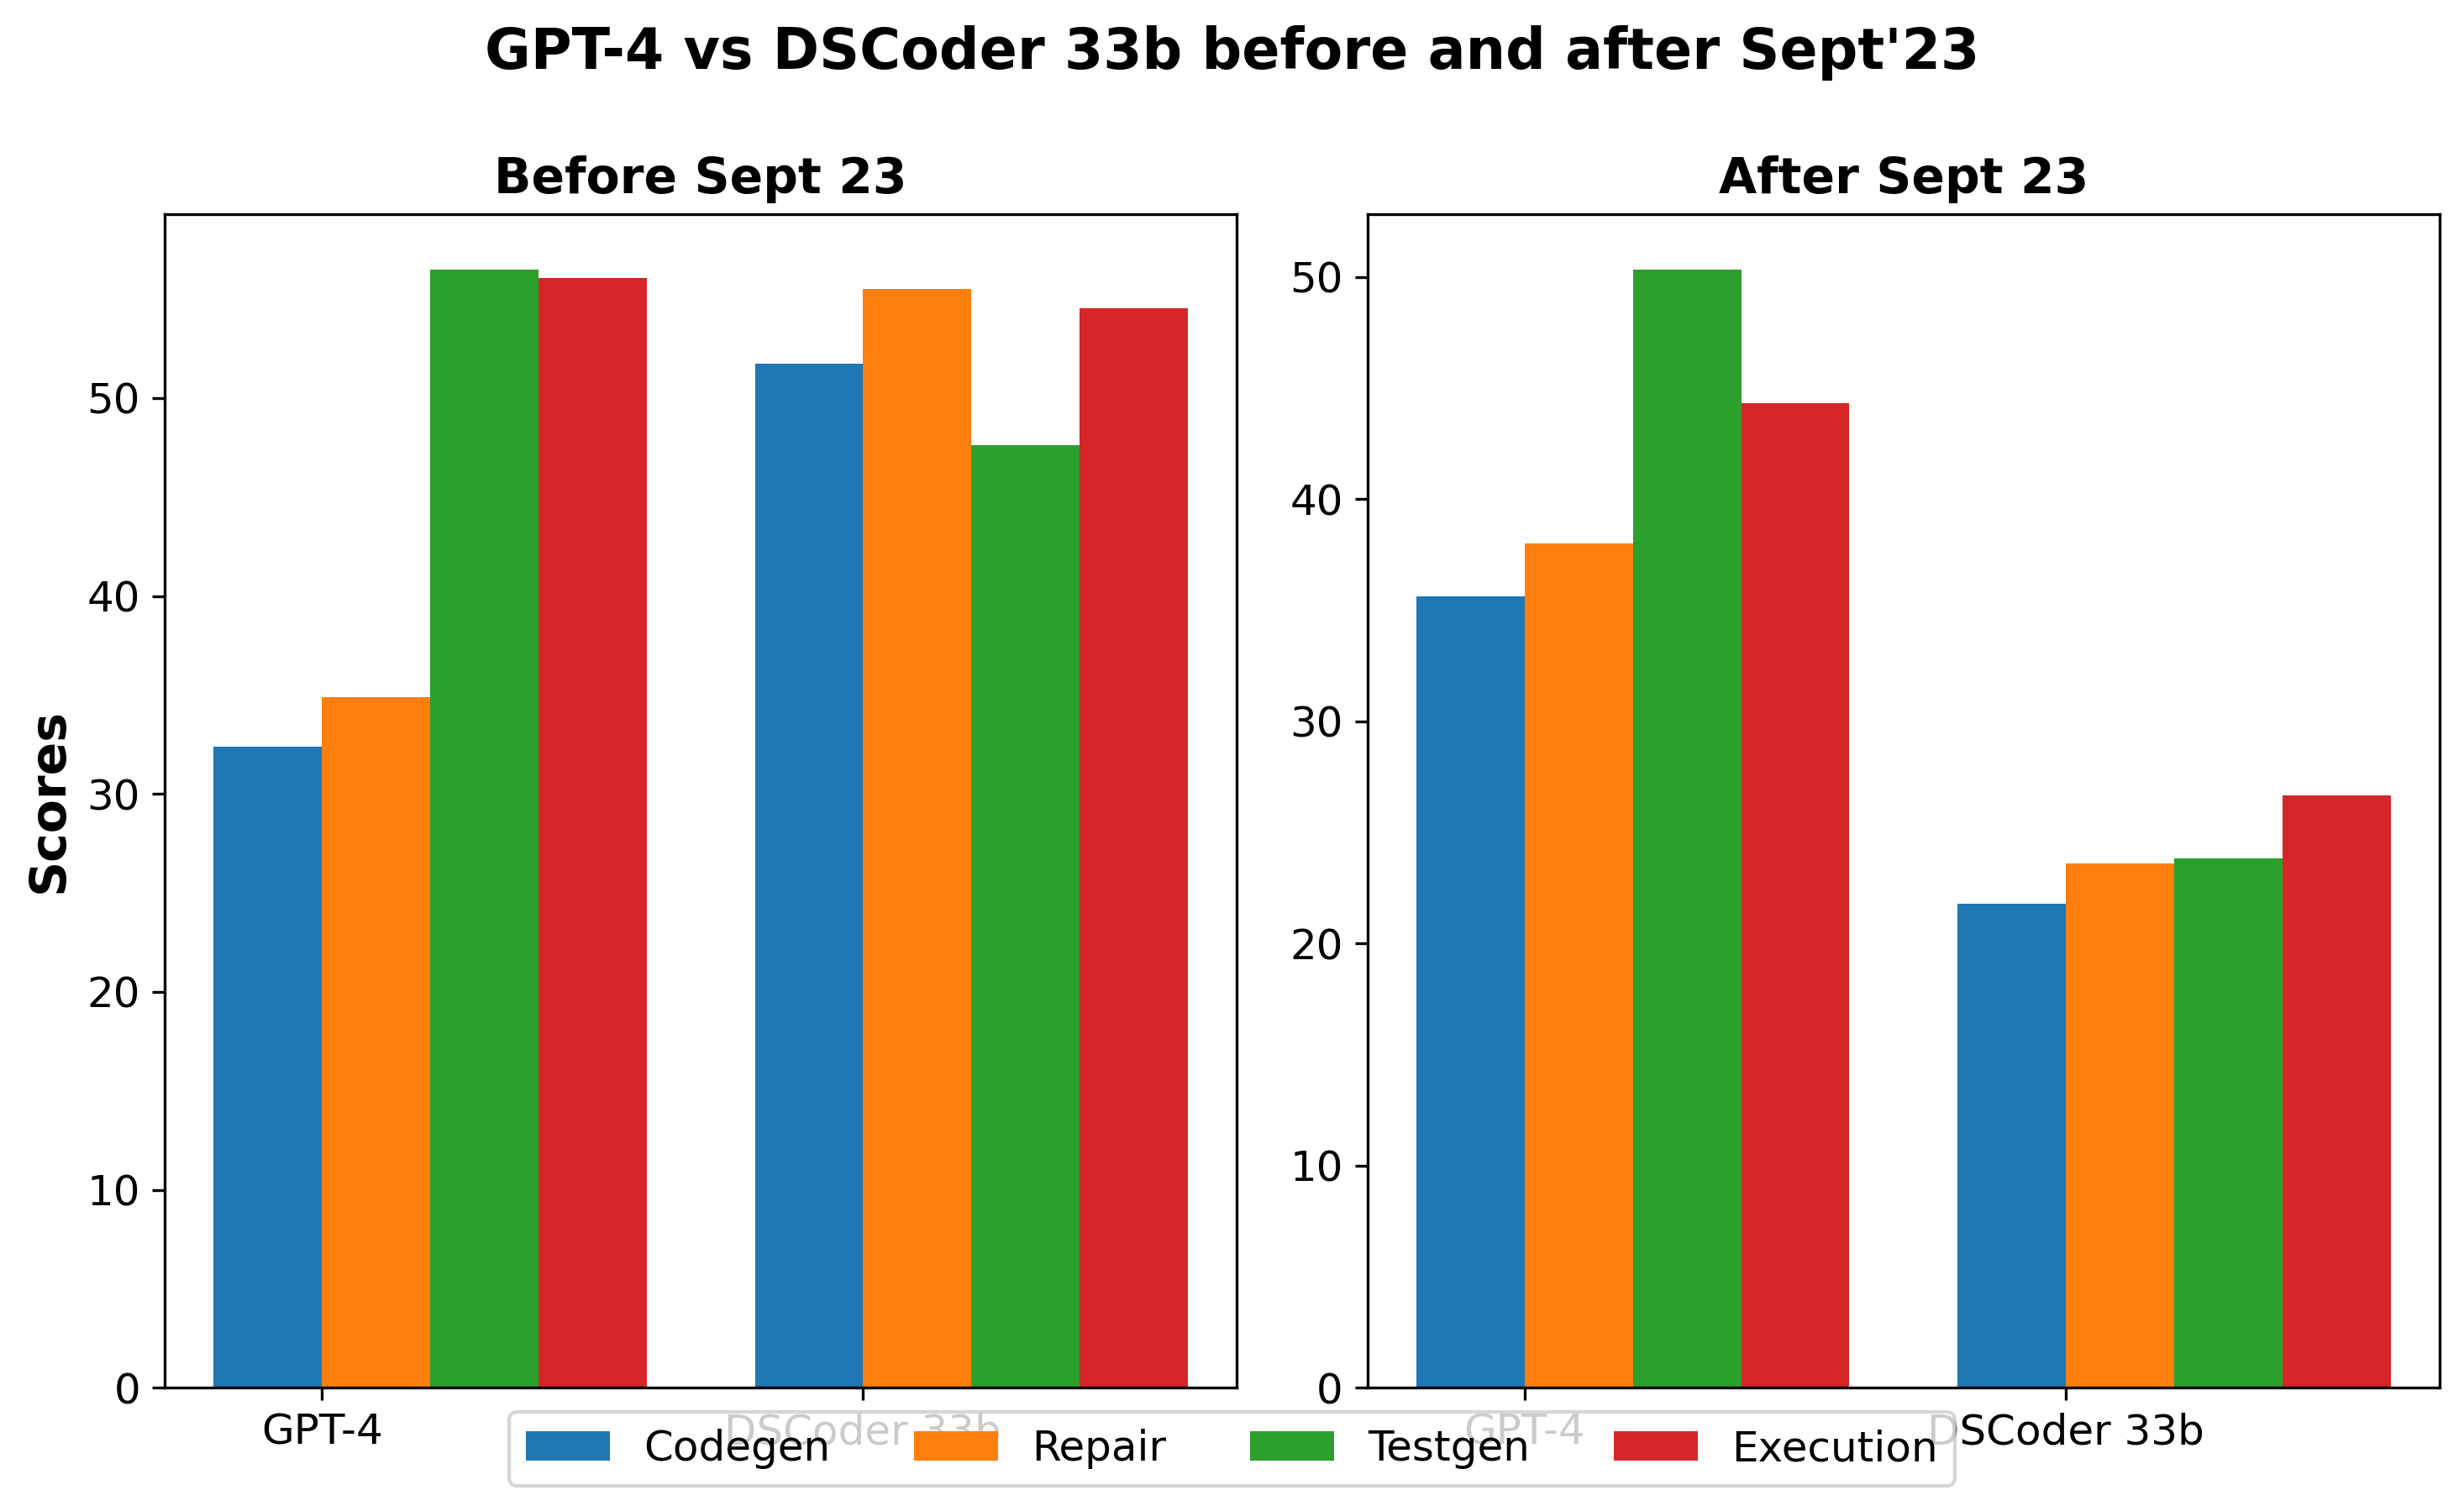
\includegraphics[width=\columnwidth]{figures/contamination/contamination_all_tasks.png}
%     \caption{Contamination in \deepseekcode{} models across different scenarios. We notice a sharp drop in performance when evaluated on \leetcode{} problems before and after September 2023.}
%     \label{fig:contamination_all_tasks}
% \end{figure}

\begin{figure}[!h]
%    
\includegraphics[width=0.49\linewidth]{figures/overview/live_evaluation_over_time.png}%
    %\hfil%
    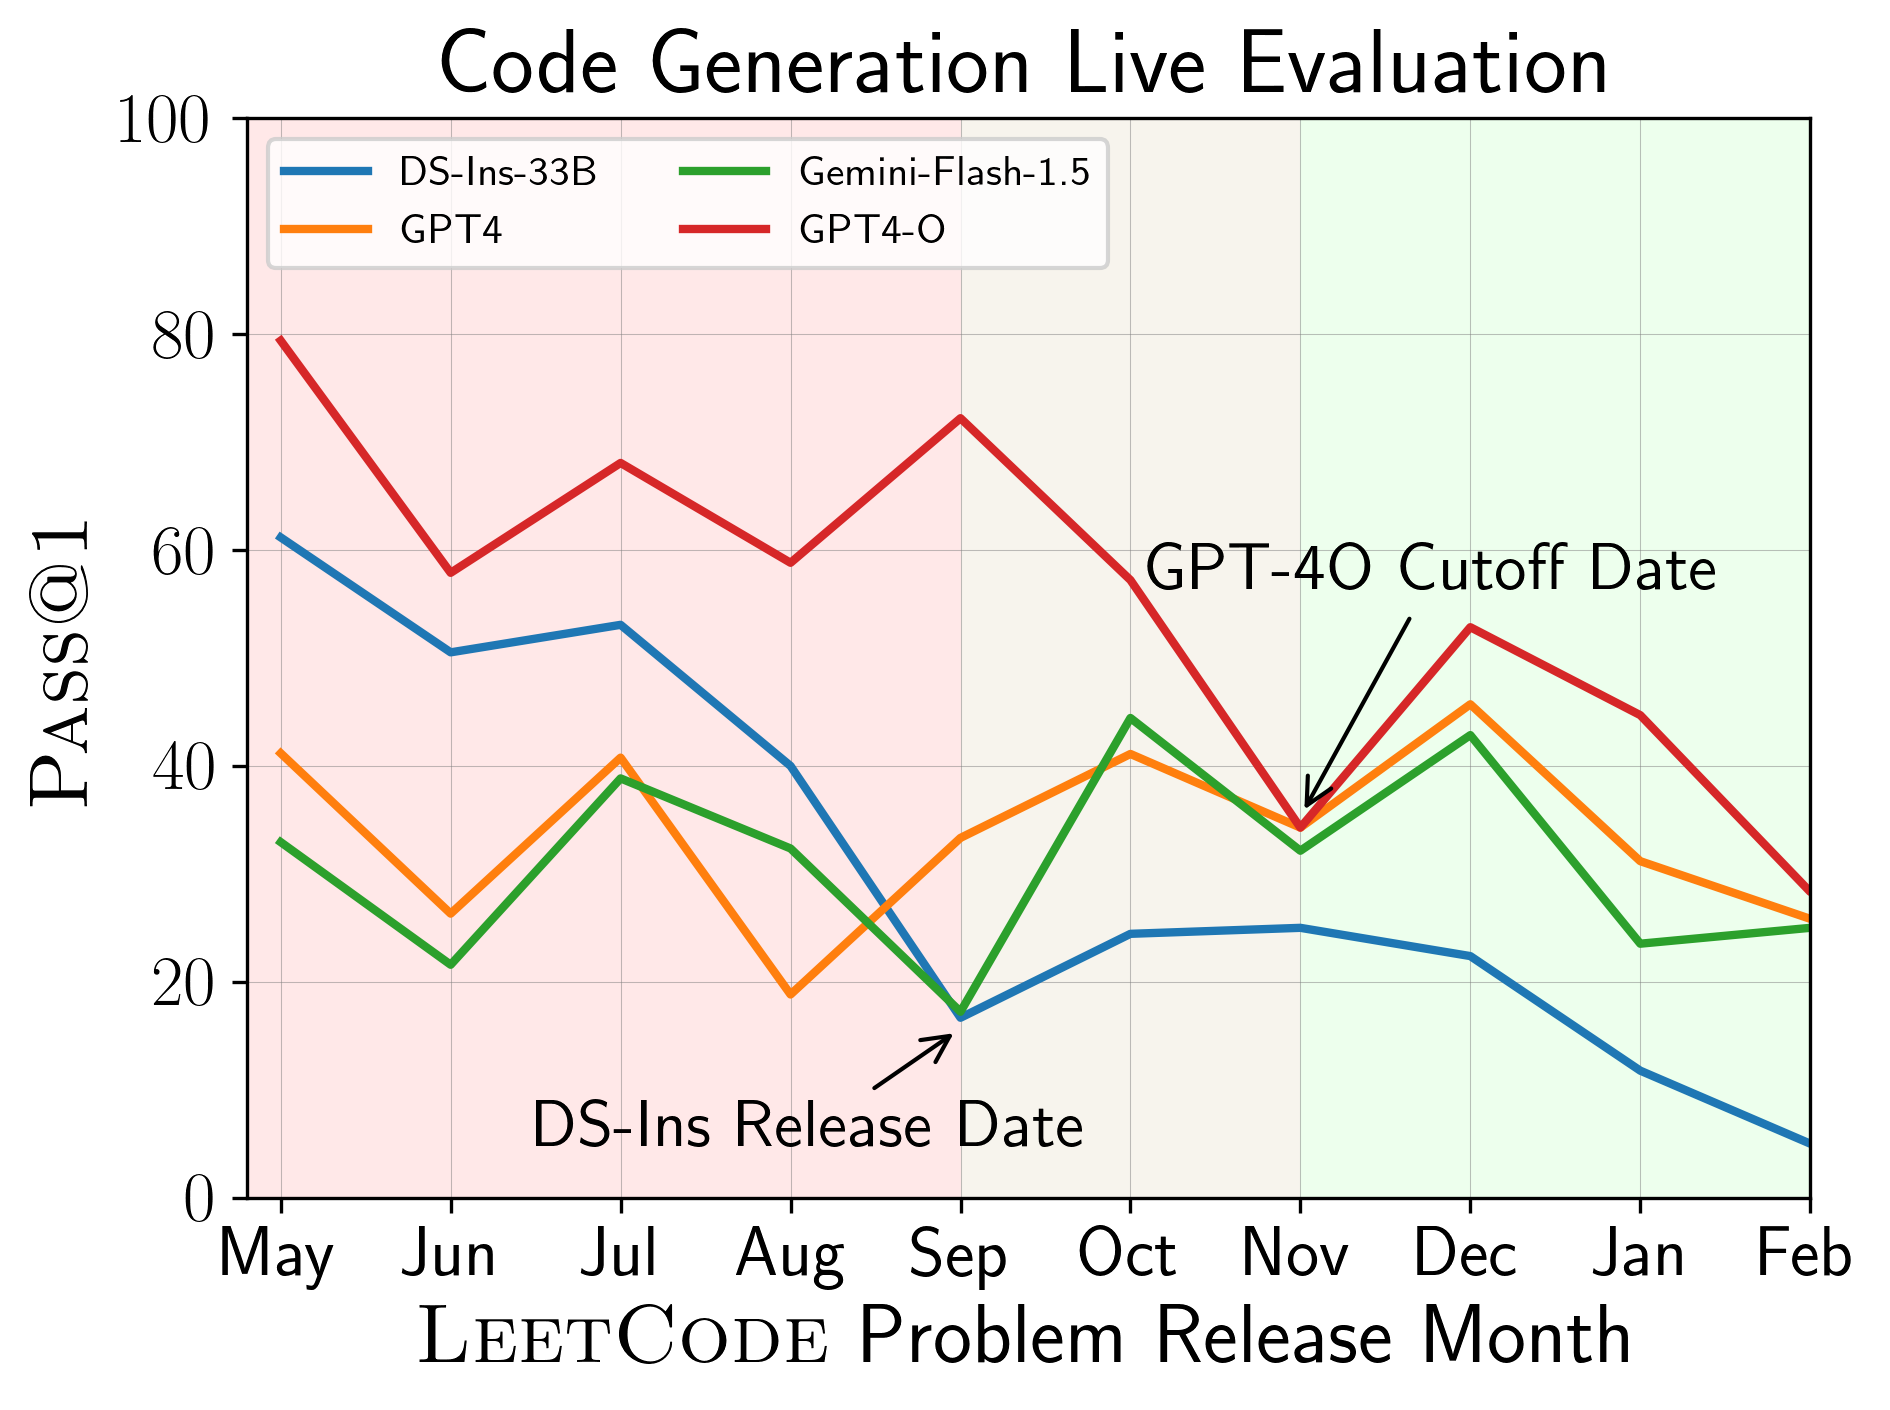
\includegraphics[width=0.49\linewidth]{figures/contamination_new/main_14_codegen_leetcode.png}
    \hfil%
    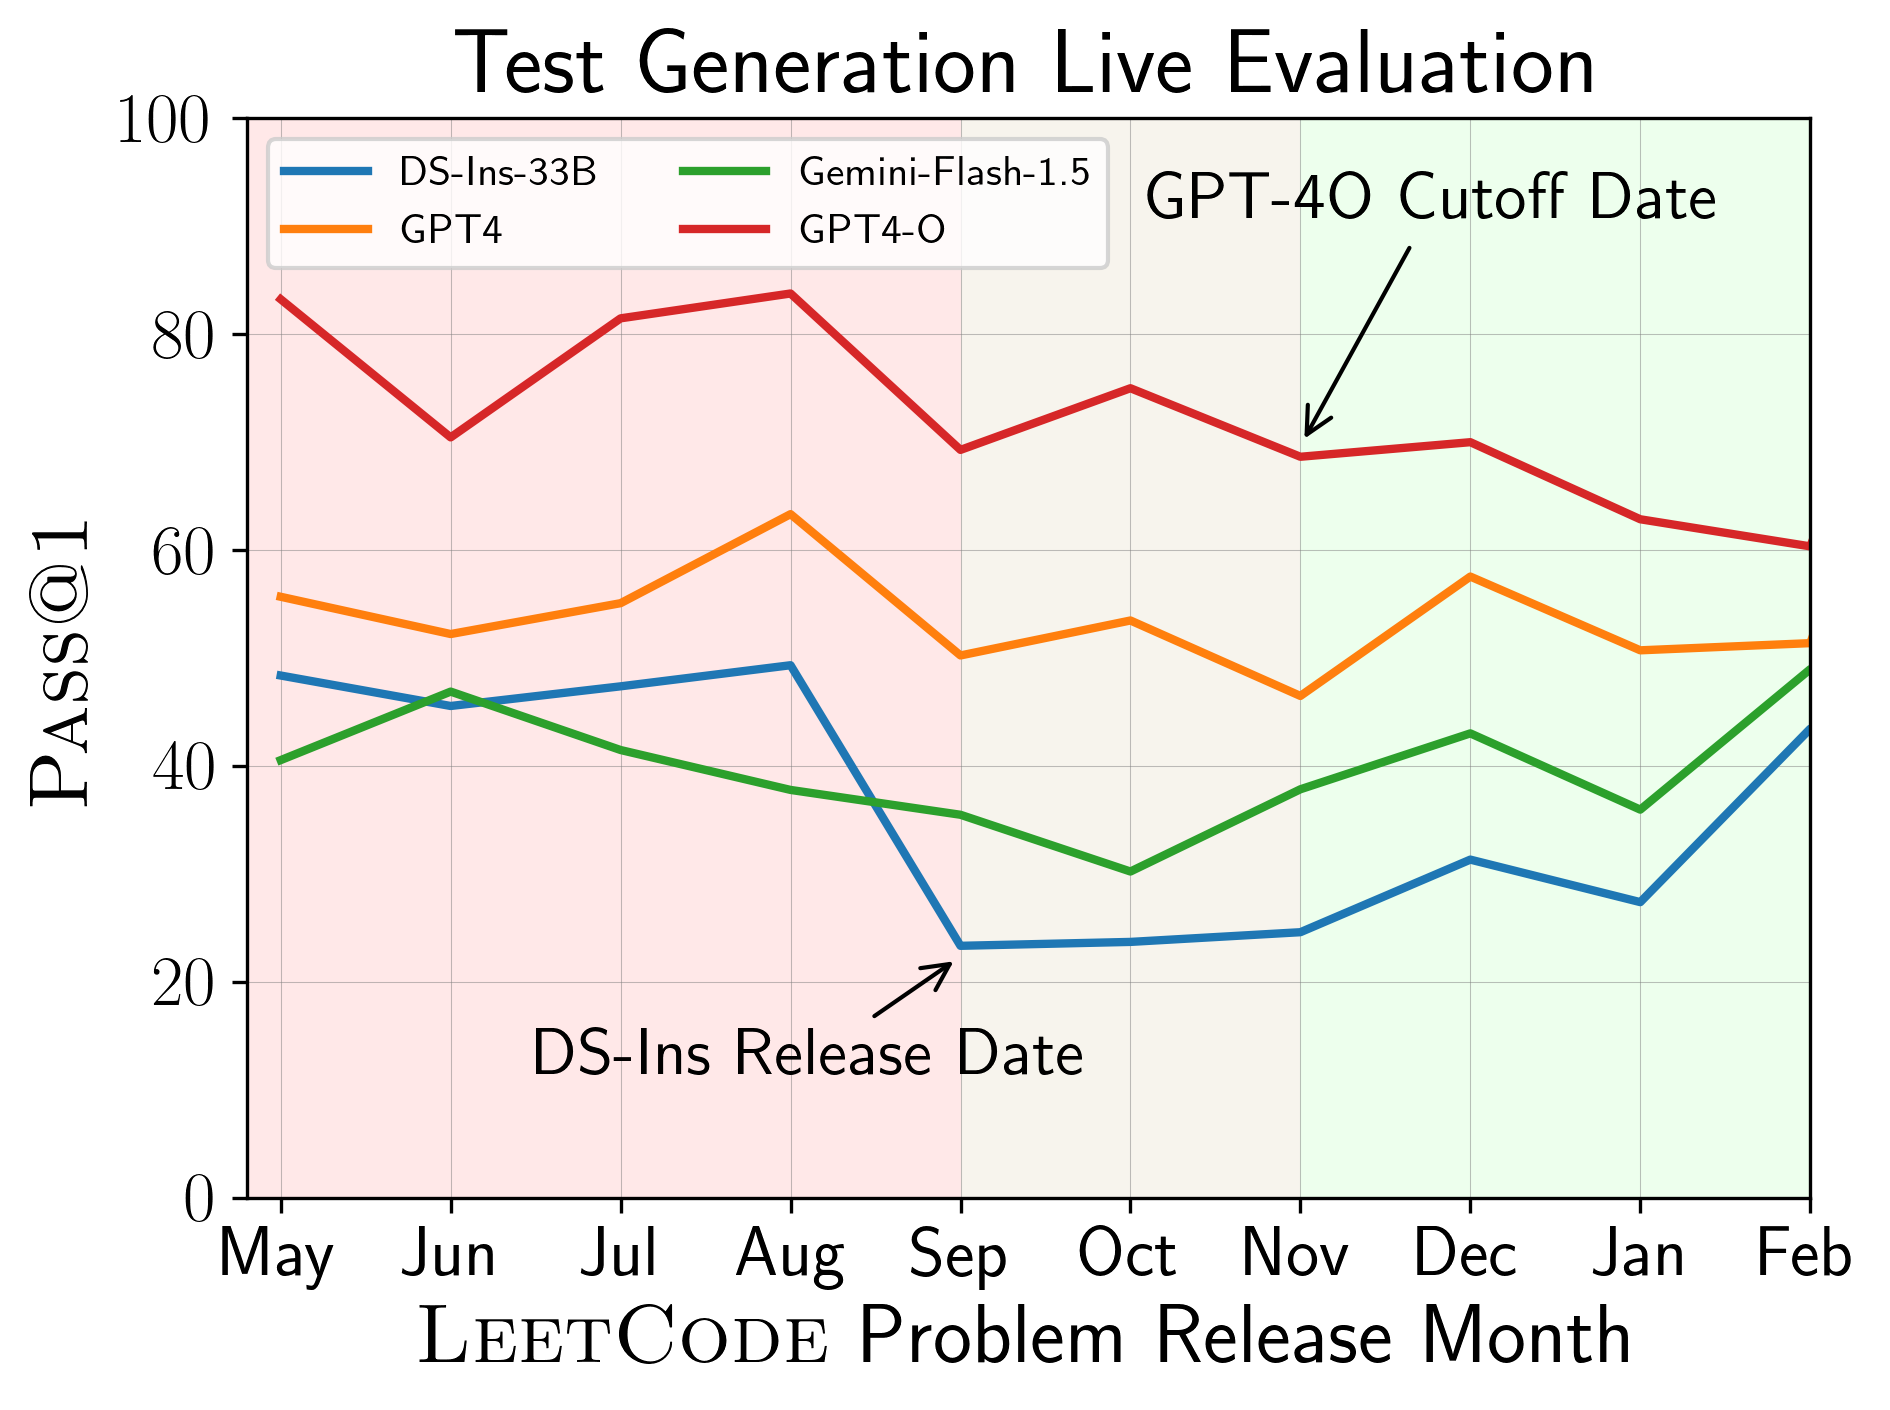
\includegraphics[width=0.49\linewidth]{figures/contamination_new/main_14_testgen_leetcode.png}
    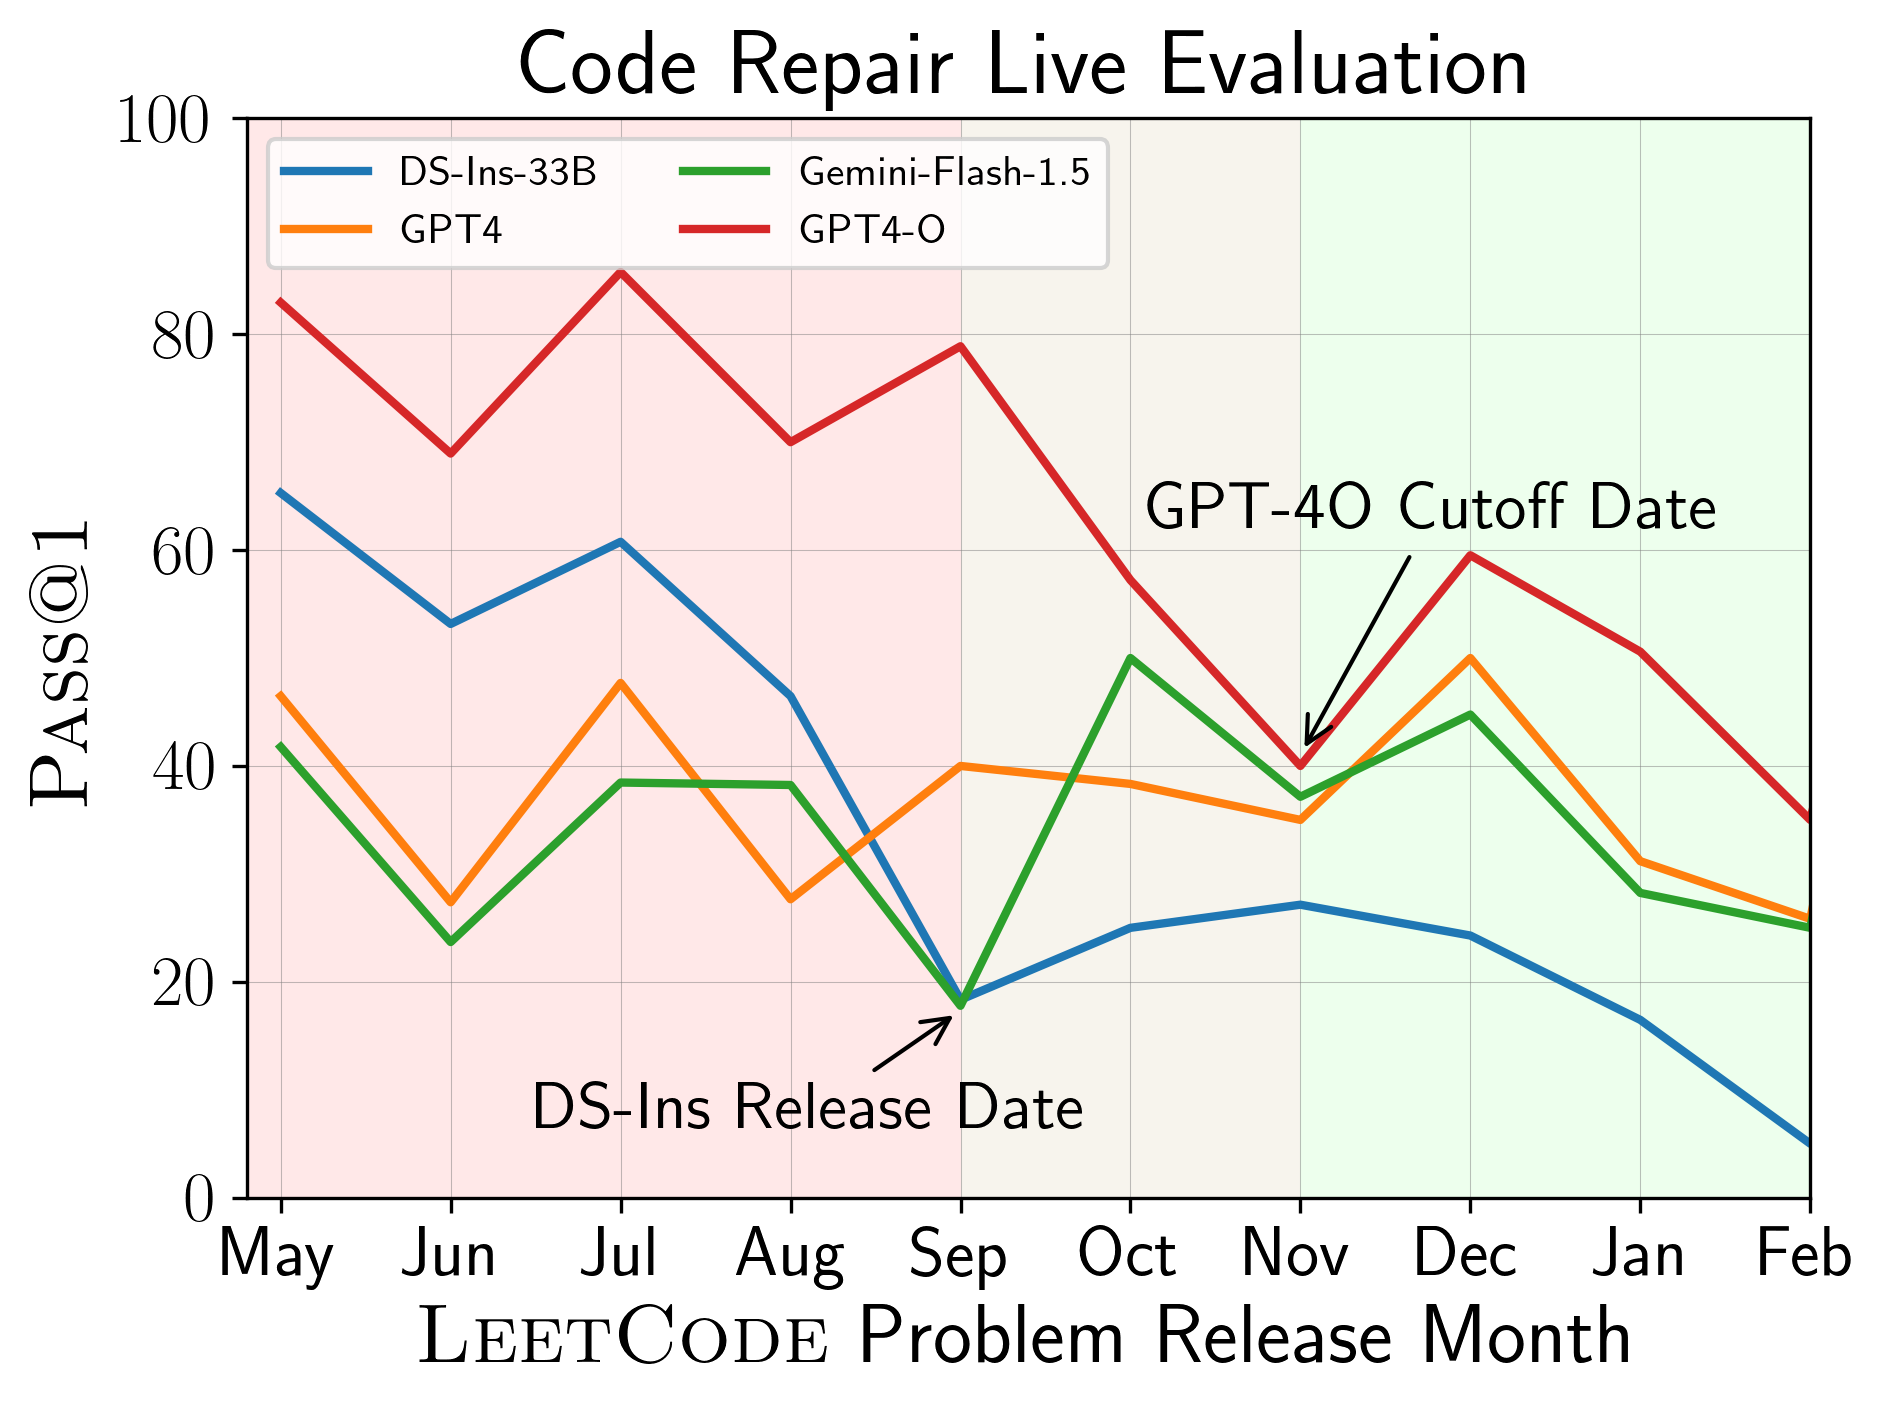
\includegraphics[width=0.49\linewidth]{figures/contamination_new/main_14_repair_leetcode.png}
    \hfil%
    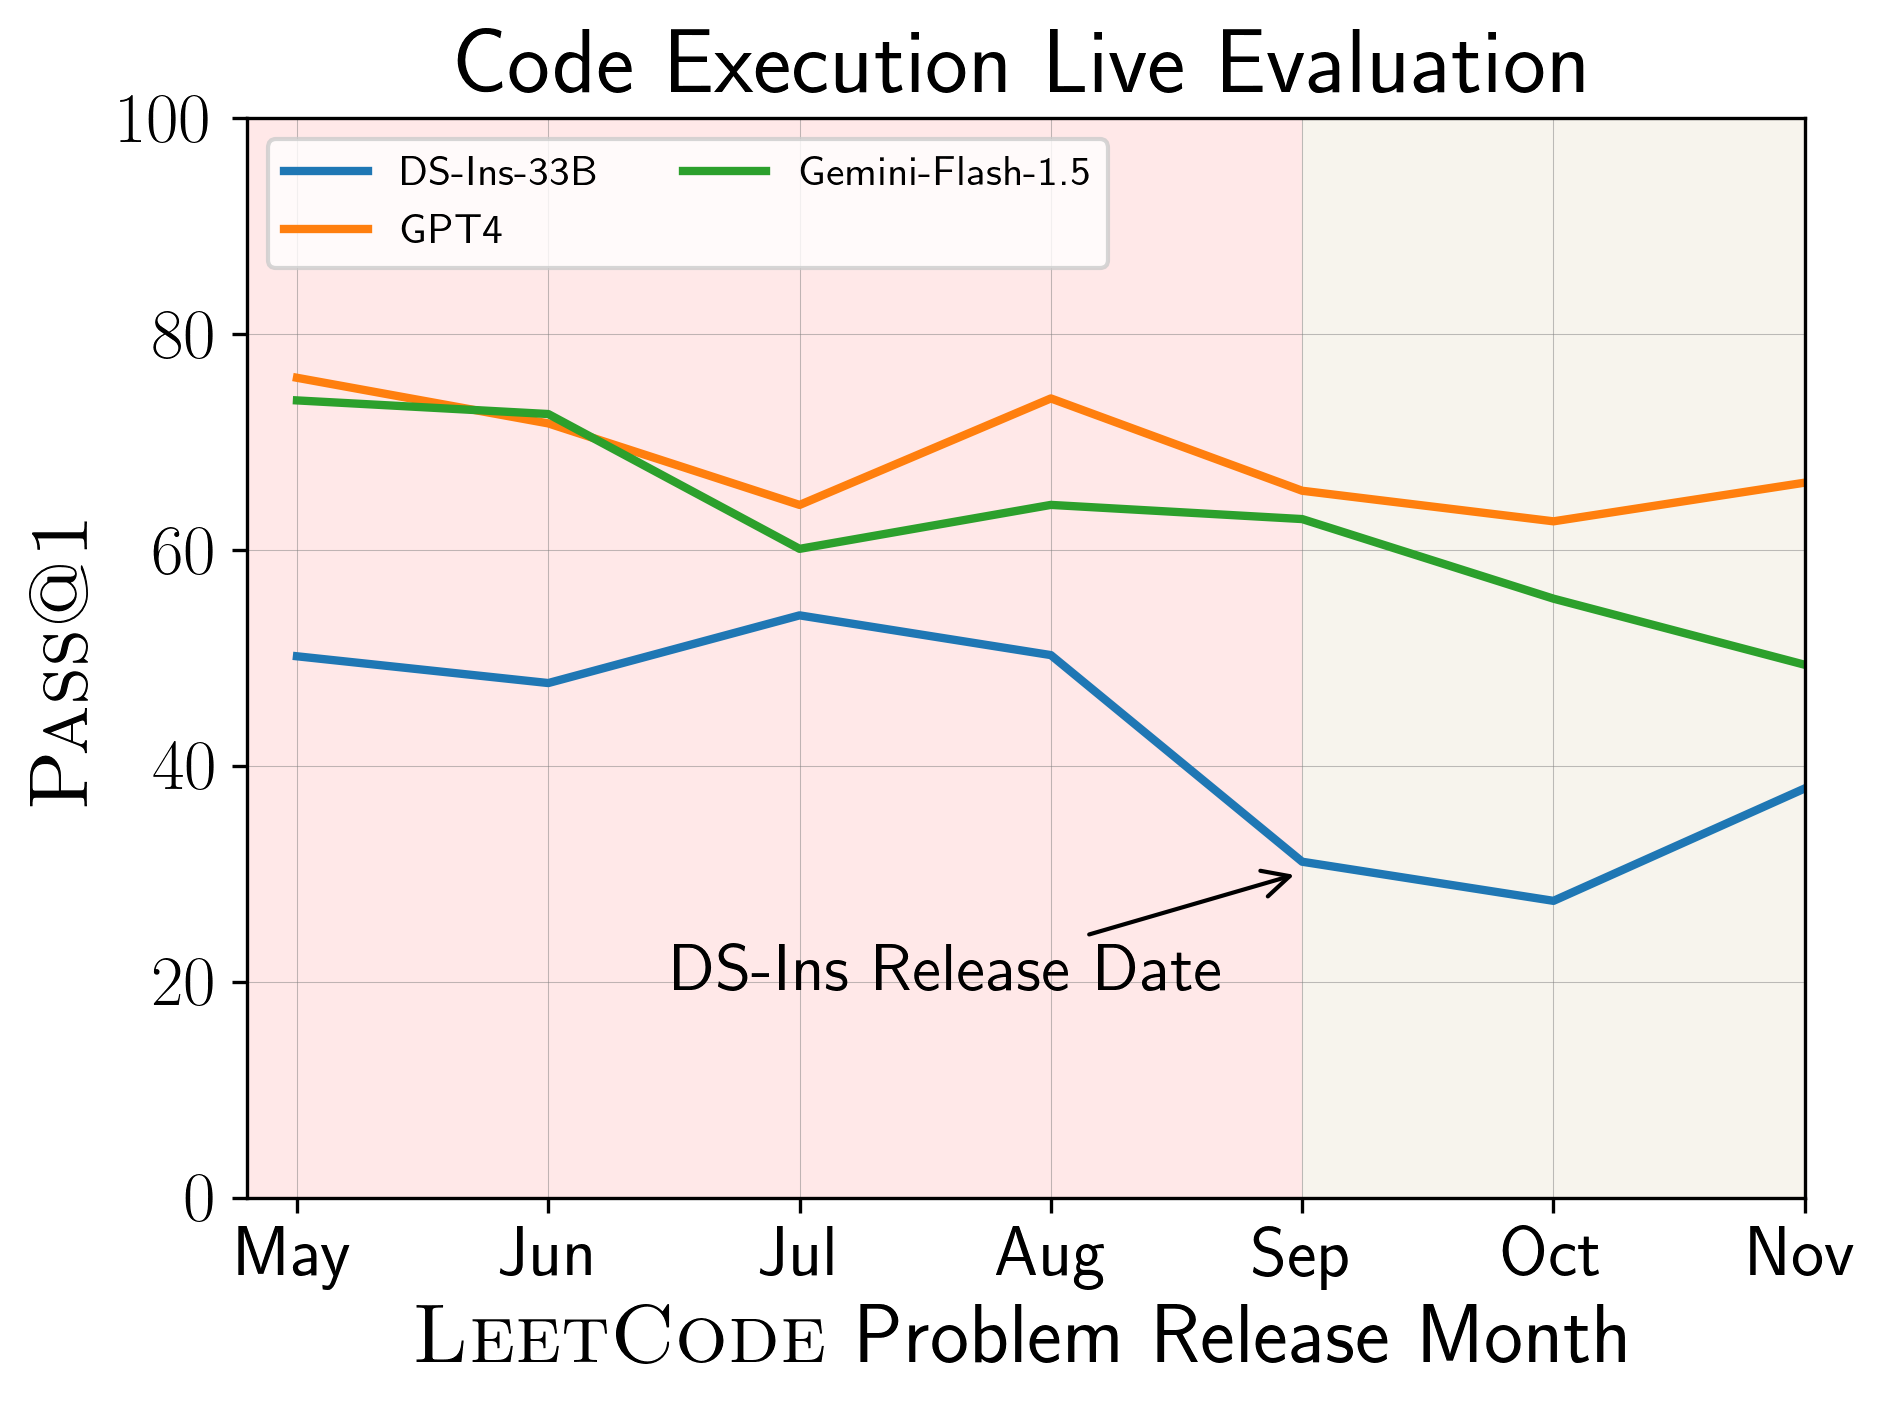
\includegraphics[width=0.49\linewidth]{figures/contamination_new/main_14_codeexec_leetcode.png}%
    
    %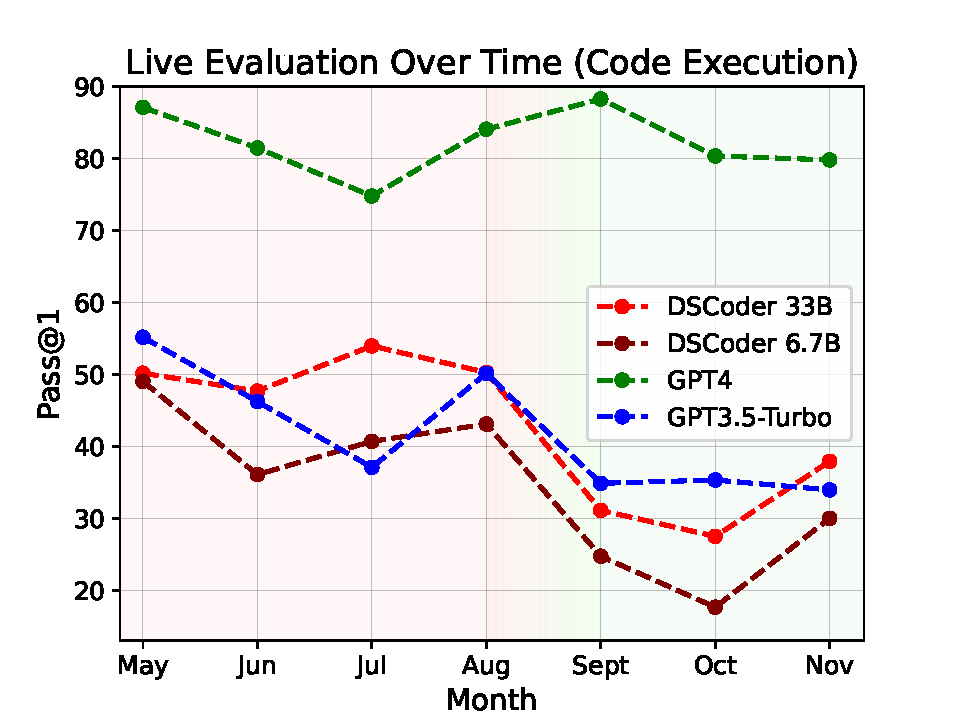
\includegraphics[width=0.49\linewidth]{figures/contamination/live_evaluation_over_time_execution.pdf}
    \caption{Contamination in \deepseekcode{} models across self-repair and code execution (without \chainot{}) scenarios over time. Note that code execution currently runs between May and November}
    \label{fig:contamination_all_tasks_line}
\end{figure}


\begin{figure}[!h]
%    
\includegraphics[width=0.49\linewidth]{figures/overview/live_evaluation_over_time.png}%
\centering
    %\hfil%
    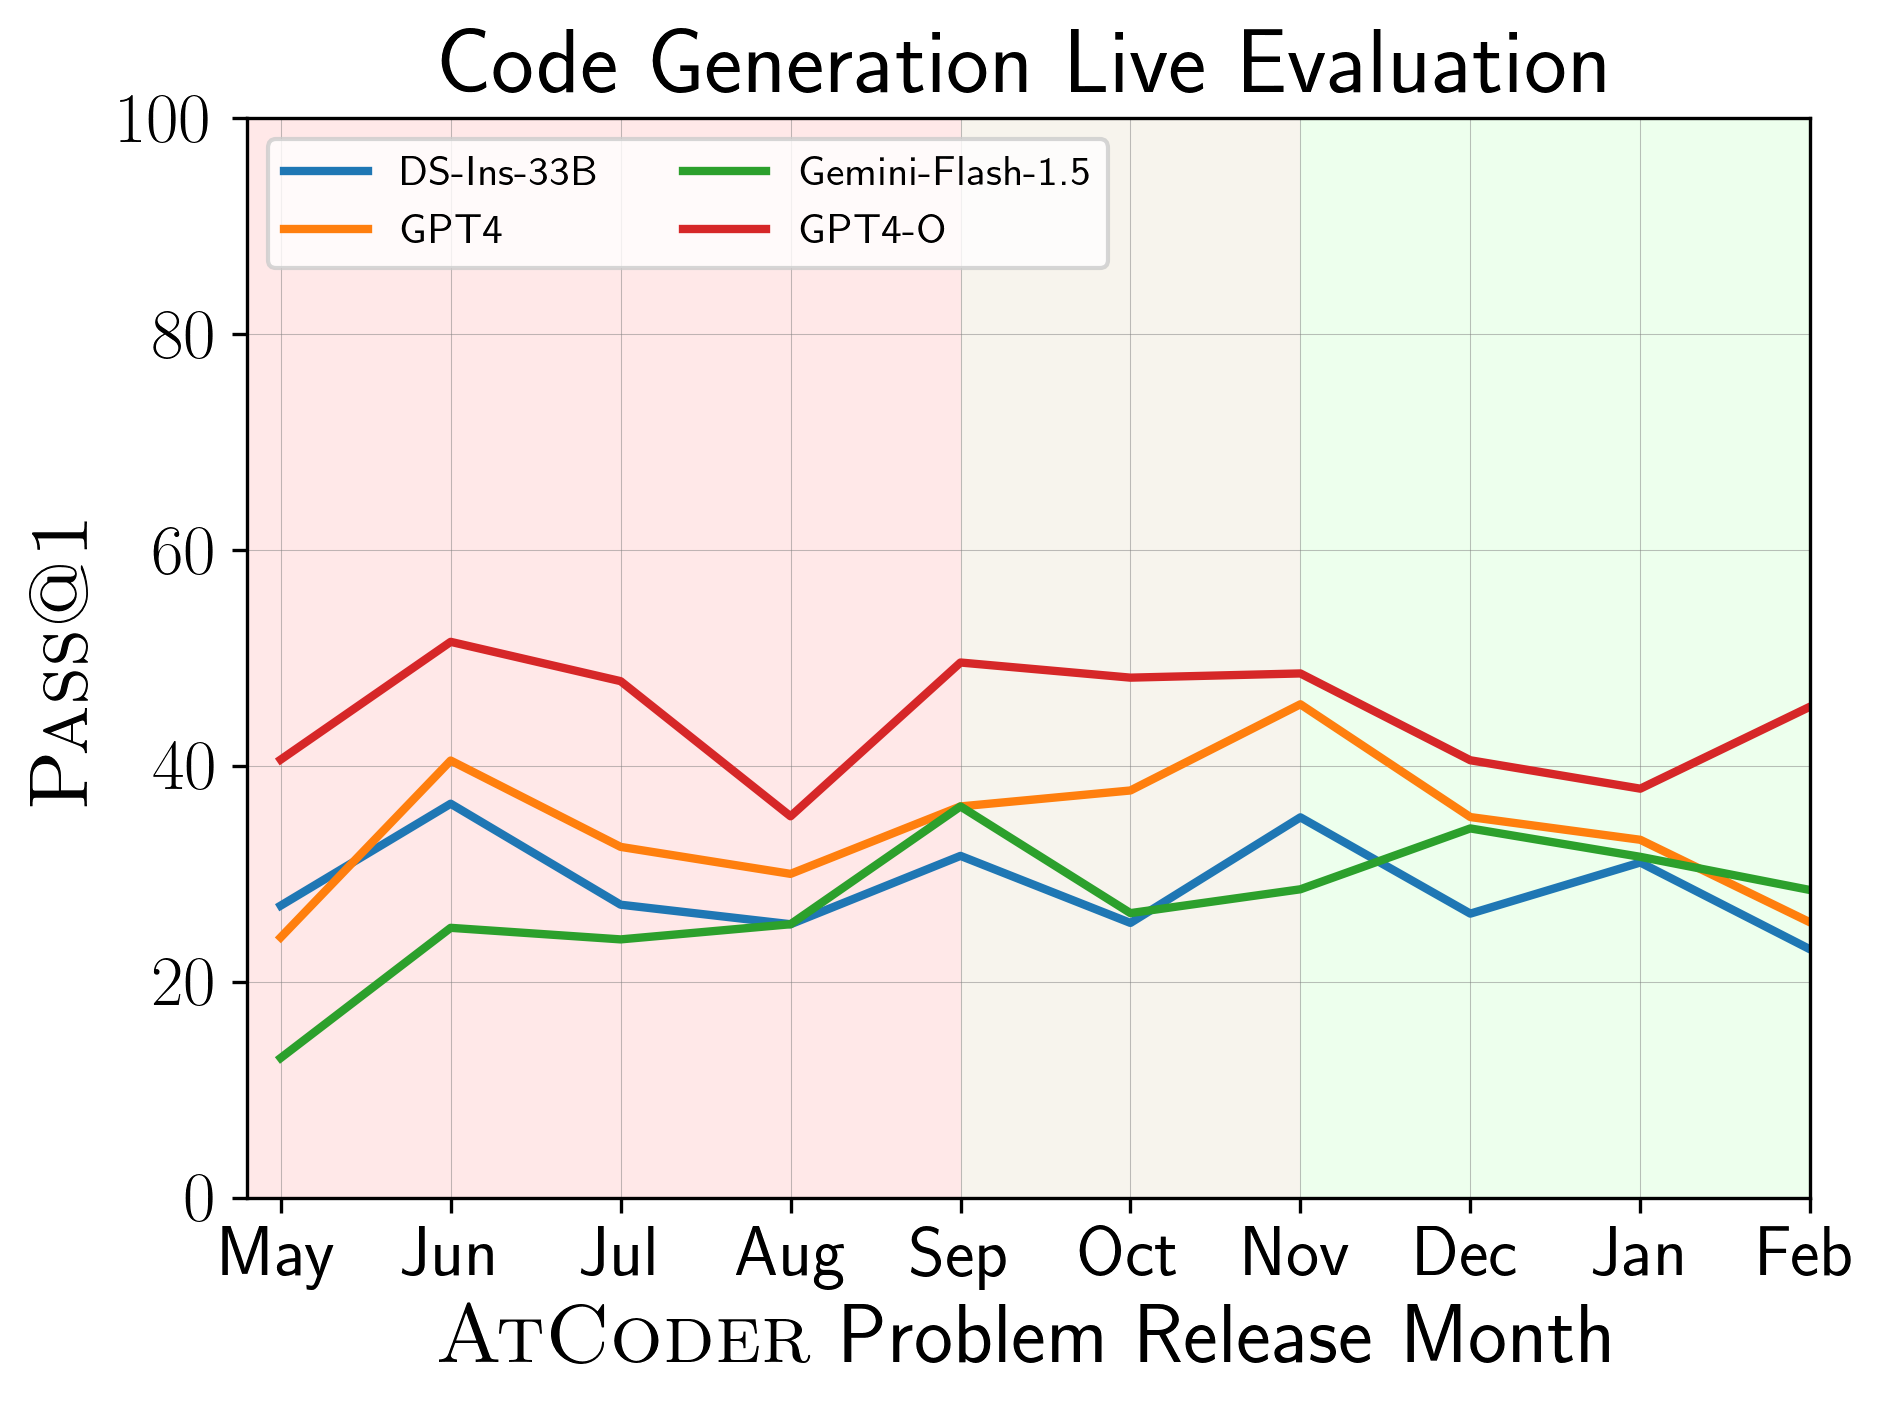
\includegraphics[width=0.49\linewidth]{figures/contamination_new/main_14_codegen_atcoder.png}
        \caption{Performance on problems released over different months for \atcoder{}}
    \label{fig:atcoder_contamination}

\end{figure}

\subsubsection{All Results}
Below we provide the tables comprising of results across different \livecodebench{} scenarios.
\begin{table}[ht]
\centering
\begin{tabular}{lrrrr}
    \hline
Model Name & Easy & Medium & Hard & Total \\
    \hline
Claude-2 & 61.80& 4.90& 0.20& 22.30\\
Claude-3-Haiku & 63.00& 4.30& 1.10& 22.80\\
Claude-3-Opus & 78.80& 16.30& 3.20& 32.80\\
Claude-3-Sonnet & 67.60& 6.20& 1.10& 25.00\\
Claude-Instant-1 & 60.70& 4.30& 1.10& 22.10\\
CodeGemma-2b-Base & 18.30& 0.40& 0.00& 6.30\\
CodeGemma-7b-Base & 35.70& 2.60& 0.10& 12.80\\
CodeLlama-13b-Base & 24.60& 0.90& 0.00& 8.50\\
CodeLlama-13b-Ins & 36.60& 2.40& 0.00& 13.00\\
CodeLlama-34b-Base & 32.20& 1.80& 0.10& 11.40\\
CodeLlama-34b-Ins & 33.70& 2.40& 1.10& 12.40\\
CodeLlama-70b-Base & 15.80& 1.20& 0.00& 5.70\\
CodeLlama-70b-Ins & 7.80& 0.60& 0.00& 2.80\\
CodeLlama-7b-Base & 19.00& 0.40& 0.00& 6.50\\
CodeLlama-7b-Ins & 28.60& 2.50& 0.00& 10.40\\
CodeQwen15-7B & 40.40& 4.80& 0.00& 15.10\\
CodeQwen15-7B-Chat & 39.20& 13.10& 0.50& 17.60\\
Codestral-Latest & 69.00& 18.70& 0.90& 29.50\\
Command-R & 39.00& 3.60& 0.00& 14.20\\
Command-R+ & 56.60& 6.80& 0.00& 21.10\\
DSCoder-1.3b-Base & 17.30& 0.70& 0.00& 6.00\\
DSCoder-1.3b-Ins & 22.90& 1.50& 0.00& 8.10\\
DSCoder-33b-Base & 39.40& 2.30& 0.00& 13.90\\
DSCoder-33b-Ins & 55.60& 9.00& 0.70& 21.80\\
DSCoder-6.7b-Base & 34.30& 1.40& 0.10& 11.90\\
DSCoder-6.7b-Ins & 46.40& 5.80& 0.70& 17.60\\
GPT-3.5-Turbo-0125 & 56.80& 10.80& 0.10& 22.60\\
GPT-3.5-Turbo-0301 & 53.40& 8.80& 0.20& 20.80\\
GPT-4-0613 & 78.40& 21.20& 2.30& 33.90\\
GPT-4-Turbo-1106 & 84.40& 24.00& 0.50& 36.30\\
GPT-4-Turbo-2024-04-09 & 85.30& 33.00& 5.10& 41.10\\
GPT-4O-2024-05-13 & 88.30& 33.20& 4.20& 41.90\\
Gemini-Flash-1.5-May & 68.10& 12.60& 2.70& 27.80\\
Gemini-Pro-1.5-April (n=1) & 56.50& 14.30& 3.60& 24.80\\
Gemini-Pro-1.5-May & 76.00& 19.40& 3.50& 33.00\\
Gemma-2b-Base & 6.10& 0.00& 0.00& 2.00\\
Gemma-7b-Base & 27.00& 0.90& 0.00& 9.30\\
LLama3-70b-Base & 52.20& 3.20& 0.60& 18.60\\
LLama3-70b-Ins & 60.70& 15.80& 1.40& 26.00\\
LLama3-8b-Base & 32.90& 1.50& 0.00& 11.50\\
LLama3-8b-Ins & 38.60& 3.50& 0.50& 14.20\\
MagiCoderS-CL-7B & 32.80& 2.40& 0.00& 11.70\\
MagiCoderS-DS-6.7B & 49.20& 7.50& 0.00& 18.90\\
Mistral-Large & 60.20& 10.90& 0.90& 24.00\\
Mixtral-8x22B-Ins & 59.80& 12.70& 0.00& 24.20\\
Mixtral-8x7B-Ins & 31.60& 2.60& 0.00& 11.40\\
OC-DS-1.3B & 11.30& 0.10& 0.00& 3.80\\
OC-DS-33B & 53.90& 5.10& 0.00& 19.70\\
OC-DS-6.7B & 46.30& 4.50& 0.00& 16.90\\
Phind-34B-V2 & 53.40& 4.70& 0.10& 19.40\\
StarCoder2-15b & 37.30& 2.20& 0.00& 13.20\\
StarCoder2-3b & 28.20& 0.70& 0.00& 9.60\\
StarCoder2-7b & 29.90& 1.20& 0.00& 10.40\\
    \hline
    \end{tabular}
\caption{Code Generation Performances}
\end{table}

\begin{table}[ht]
\centering
\begin{tabular}{lrrrr}
    \hline
Model Name & Easy & Medium & Hard & Total \\
    \hline
Claude-2 & 66.20& 10.30& 0.40& 25.60\\
Claude-3-Haiku & 66.50& 8.70& 2.50& 25.90\\
Claude-3-Opus & 83.10& 23.70& 6.70& 37.80\\
Claude-3-Sonnet & 72.60& 11.80& 2.20& 28.90\\
Claude-Instant-1 & 64.40& 7.10& 2.20& 24.60\\
CodeLlama-13b-Ins & 43.10& 3.00& 0.00& 15.30\\
CodeLlama-34b-Ins & 31.50& 3.50& 1.80& 12.30\\
CodeLlama-7b-Ins & 31.90& 3.10& 1.50& 12.10\\
Codestral-Latest & 72.50& 25.90& 3.30& 33.90\\
DSCoder-1.3b-Ins & 29.50& 2.10& 0.00& 10.60\\
DSCoder-33b-Ins & 60.70& 8.10& 1.50& 23.40\\
DSCoder-6.7b-Ins & 49.90& 5.70& 1.10& 18.90\\
GPT-3.5-Turbo-0125 & 59.30& 11.90& 0.50& 23.90\\
GPT-3.5-Turbo-0301 & 58.40& 11.60& 0.70& 23.60\\
GPT-4-0613 & 79.30& 25.00& 2.40& 35.60\\
GPT-4-Turbo-1106 & 86.90& 36.90& 4.00& 42.60\\
GPT-4-Turbo-2024-04-09 & 88.70& 39.70& 8.40& 45.60\\
GPT-4O-2024-05-13 & 92.60& 46.40& 8.20& 49.10\\
Gemini-Flash-1.5-May & 73.40& 16.40& 4.40& 31.40\\
Gemini-Pro & 53.80& 9.40& 0.20& 21.10\\
Gemini-Pro-1.5-April (n=1) & 71.80& 19.40& 5.50& 32.20\\
Gemini-Pro-1.5-May & 84.80& 30.10& 7.30& 40.70\\
LLama3-70b-Ins & 69.60& 19.00& 1.80& 30.10\\
LLama3-8b-Ins & 47.10& 6.10& 0.00& 17.70\\
MagiCoderS-CL-7B & 36.50& 3.10& 0.00& 13.20\\
MagiCoderS-DS-6.7B & 50.60& 8.60& 0.00& 19.70\\
Mistral-Large & 71.20& 15.60& 3.60& 30.10\\
OC-DS-1.3B & 20.00& 0.40& 0.00& 6.80\\
OC-DS-33B & 58.90& 7.20& 1.30& 22.50\\
OC-DS-6.7B & 50.90& 6.30& 0.20& 19.10\\
Phind-34B-V2 & 62.00& 6.50& 0.90& 23.10\\
    \hline
\end{tabular}
\caption{Self Repair Performances}
\end{table}

\begin{table}[ht]
\centering
\begin{tabular}{lr}
    \hline
Model Name & Pass@1 \\
    \hline
Claude-2 & 32.70\\
Claude-3-Haiku & 32.90\\
Claude-3-Opus & 58.70\\
Claude-3-Sonnet & 34.10\\
Claude-Instant-1 & 25.40\\
CodeLlama-13b-Ins & 24.40\\
CodeLlama-34b-Ins & 23.00\\
CodeLlama-70b-Ins & 16.10\\
CodeLlama-7b-Ins & 15.30\\
Codestral-Latest & 41.80\\
DSCoder-1.3b-Ins & 12.50\\
DSCoder-33b-Ins & 28.30\\
DSCoder-6.7b-Ins & 26.50\\
GPT-3.5-Turbo-0125 & 35.40\\
GPT-3.5-Turbo-0301 & 32.50\\
GPT-4-0613 & 52.90\\
GPT-4-Turbo-1106 & 55.70\\
GPT-4-Turbo-2024-04-09 & 66.10\\
GPT-4O-2024-05-13 & 68.90\\
Gemini-Flash-1.5-May & 38.10\\
Gemini-Pro & 29.50\\
Gemini-Pro-1.5-April (n=1) & 49.60\\
Gemini-Pro-1.5-May & 44.80\\
LLama3-70b-Ins & 41.40\\
LLama3-8b-Ins & 24.40\\
MagiCoderS-CL-7B & 21.30\\
MagiCoderS-DS-6.7B & 27.10\\
Mistral-Large & 46.50\\
Mixtral-8x22B-Ins & 44.70\\
Mixtral-8x7B-Ins & 31.80\\
OC-DS-1.3B & 7.80\\
OC-DS-33B & 11.30\\
OC-DS-6.7B & 18.30\\
Phind-34B-V2 & 27.20\\
    \hline
\end{tabular}
\caption{Test Output Prediction Performances}
\end{table}

\begin{table}[ht]
\centering
\begin{tabular}{lrr}
    \hline
Model Name & Pass@1 & Pass@1 (COT) \\
    \hline
Claude-2 & 31.50 & 43.80 \\
Claude-3-Haiku & 0.70 & 28.30 \\
Claude-3-Opus & 36.50 & 80.10 \\
Claude-3-Sonnet & 29.30 & 39.40 \\
Claude-Instant-1 & 20.00 & 34.80 \\
Cllama-13b-Ins & 23.50 & 14.10 \\
Cllama-34b-Ins & 28.90 & 24.50 \\
Cllama-7b-Ins & 20.60 & 14.20 \\
CodeLlama-70b-Ins & 31.20 & -1.00 \\
Codestral-Latest & 37.90 & 41.80 \\
DSCoder-1.3b-Base & 19.00 & 13.40 \\
DSCoder-1.3b-Ins & 18.10 & 17.00 \\
DSCoder-33b-Base & 29.90 & 29.10 \\
DSCoder-33b-Ins & 26.60 & 31.70 \\
DSCoder-6.7b-Base & 23.50 & 25.10 \\
DSCoder-6.7b-Ins & 23.10 & 23.80 \\
GPT-3.5-Turbo-0301 & 33.90 & 34.80 \\
GPT-4-0613 & 44.30 & 64.80 \\
GPT-4-Turbo-1106 & 40.50 & 83.60 \\
GPT-4-Turbo-2024-04-09 & 45.90 & 83.80 \\
GPT-4O-2024-05-13 & 39.10 & 91.00 \\
Gemini-Flash-1.5-May & 21.40 & 57.10 \\
Gemini-Pro & 27.70 & 37.40 \\
Gemini-Pro-1.5 (April) (n=1) & 30.30 & 64.40 \\
Gemini-Pro-1.5-May & 42.10 & 72.10 \\
LLama3-70b-Ins & 29.60 & 55.50 \\
LLama3-8b-Ins & 18.40 & 29.40 \\
MagiCoderS-CL-7B & 21.20 & -1.00 \\
MagiCoderS-DS-6.7B & 27.20 & -1.00 \\
Mistral-Large & 36.60 & 54.40 \\
Phind-34B-V2 & 26.90 & -1.00 \\
StarCoder & 20.30 & -1.00 \\
WCoder-34B-V1 & 28.40 & -1.00 \\
    \hline
\end{tabular}
\caption{Code Execution Performances}
\end{table}

%  \subsubsection{Code Execution}
% In Table \ref{tab:execution-full}, we show the results of the code execution task. We only test CoT on a subset of the instruct models. For base models, we find that CoT generally does not lead to improvements.

% \begin{table}[h]
% \centering
% \begin{tabular}{lcc}
% \toprule
% Model Name &  pass@1 & pass@1 (CoT) \\
% \midrule
% starcoderbase-7b               &  23.6 & - \\
% starcoder-16b                  &  24.7 & - \\
% phi-1                          &  25.1 & - \\
% starcoderbase-16b              &  28.0 & - \\
% codellama-7b                   &  28.6 & - \\
% phi-1.5                        &  28.7 & - \\
% deepseek-instruct-1.3b         &  28.8 & - \\
% magicoder-cl-7b                &  31.0 & - \\
% mistral-7b                     &  31.0 & - \\
% codellama-13b                  &  31.2 & - \\
% codellama-python-7b            &  31.3 & - \\
% google-gemini-pro              &  31.4 & 41.7 \\
% codellama-python-34b           &  32.3 & - \\
% deepseek-base-1.3b             &  32.6 & - \\
% phi-2                          &  32.9 & - \\
% % wizard-34b                     &  34.1 & - \\
% mixtral-8x7b                   &  34.4 & - \\
% % wizard-13b                     &  34.5 & - \\
% codellama-python-13b           &  34.9 & - \\
% phind                          &  35.0 & - \\
% claude-instant-1               &  35.8 & 43.8 \\
% codellama-34b                  &  35.8 & - \\
% codetulu-2-34b                 &  37.8 & 39.1 \\
% magicoder-ds-6.7b              &  40.1 & - \\
% deepseek-instruct-6.7b         &  40.2 & - \\
% gpt-3.5-turbo-0613             &  42.0 & 41.9 \\
% claude-2                       &  42.8 & 48.5 \\
% deepseek-instruct-33b          &  43.6 & 43.3 \\
% deepseek-base-6.7b             &  44.9 & - \\
% deepseek-base-33b              &  49.0 & 44.8 \\
% gpt-4-1106-preview             &  49.8 & 82.2 \\
% gpt-4-0613                     &  51.4 & 68.6 \\
% \bottomrule
% \end{tabular}
% \caption{Code Execution Results}
% \label{tab:execution-full}
% \end{table}

% % \begin{table}[h]
% % \centering
% % \begin{tabular}{lr}
% % \toprule
% % Model Name &  pass@1 \\
% % \midrule
% % codellama-13b+cot              &  18.1 \\
% % codellama-7b+cot               &  18.2 \\
% % mistral-7b+cot                 &  24.9 \\
% % deepseek-base-1.3b+cot         &  25.2 \\
% % deepseek-instruct-1.3b+cot     &  26.1 \\
% % codellama-34b+cot              &  29.1 \\
% % deepseek-instruct-6.7b+cot     &  34.9 \\
% % deepseek-base-6.7b+cot         &  35.7 \\
% % magicoder-ds-7b+cot            &  36.9 \\
% % codetulu-2-34b+cot             &  39.1 \\
% % google-gemini-pro+cot          &  41.7 \\
% % gpt-3.5-turbo-0613+cot         &  41.9 \\
% % deepseek-instruct-33b+cot      &  43.3 \\
% % claude-instant-1+cot           &  43.8 \\
% % deepseek-base-33b+cot          &  44.8 \\
% % claude-2+cot                   &  48.5 \\
% % gpt-4-0613+cot                 &  68.6 \\
% % gpt-4-1106-preview+cot         &  82.2 \\
% % \bottomrule
% % \end{tabular}
% % \caption{Code Execution Results with CoT}
% % \label{tab:execution-cot}
% % \end{table}

\begin{figure}[!h]
    \centering
    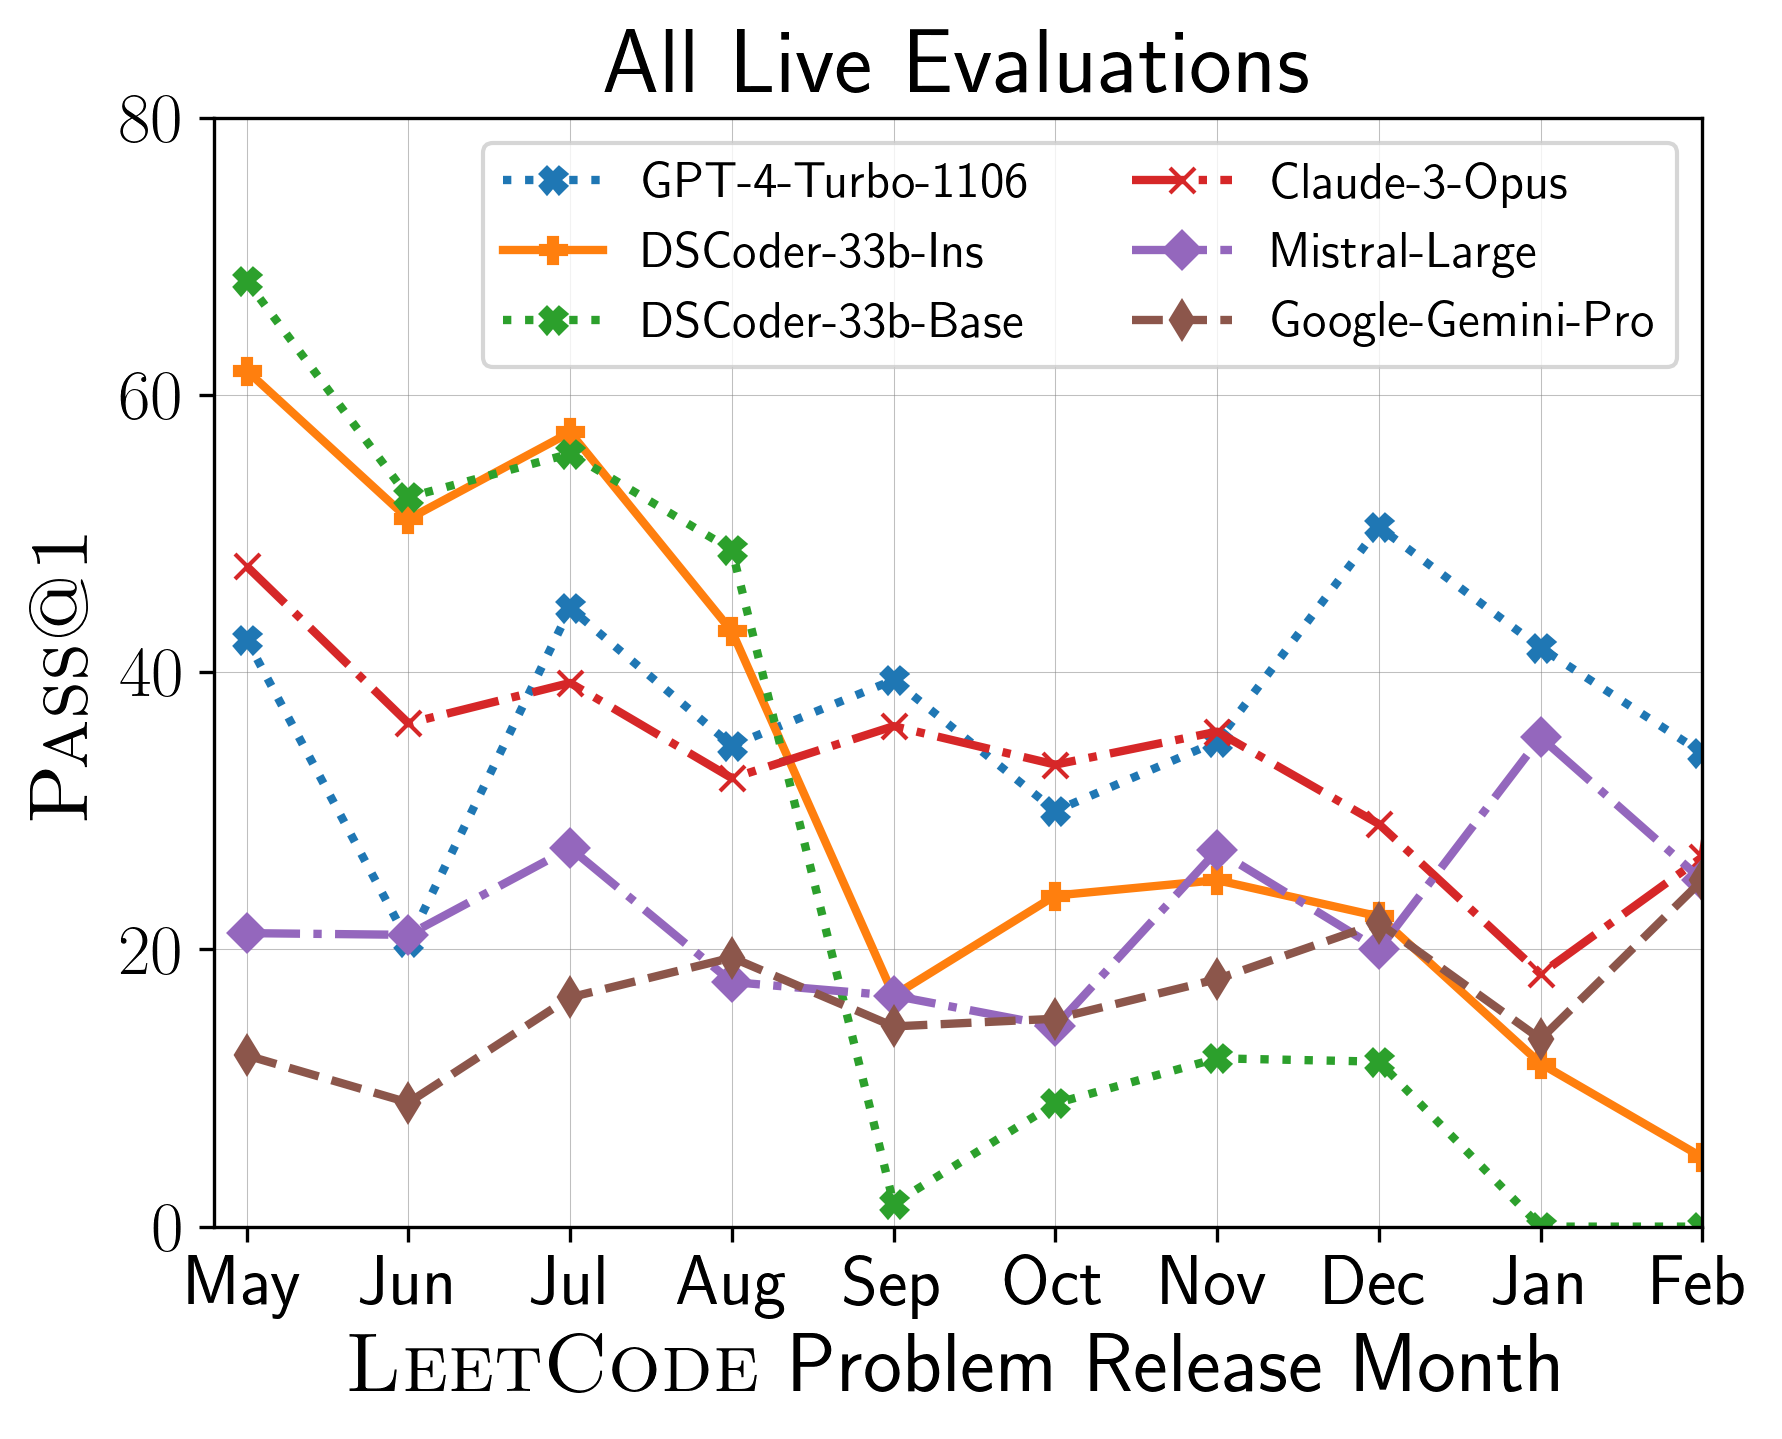
\includegraphics[width=0.49\linewidth]{figures/appendix/live_eval_custom_leetcode.png}
    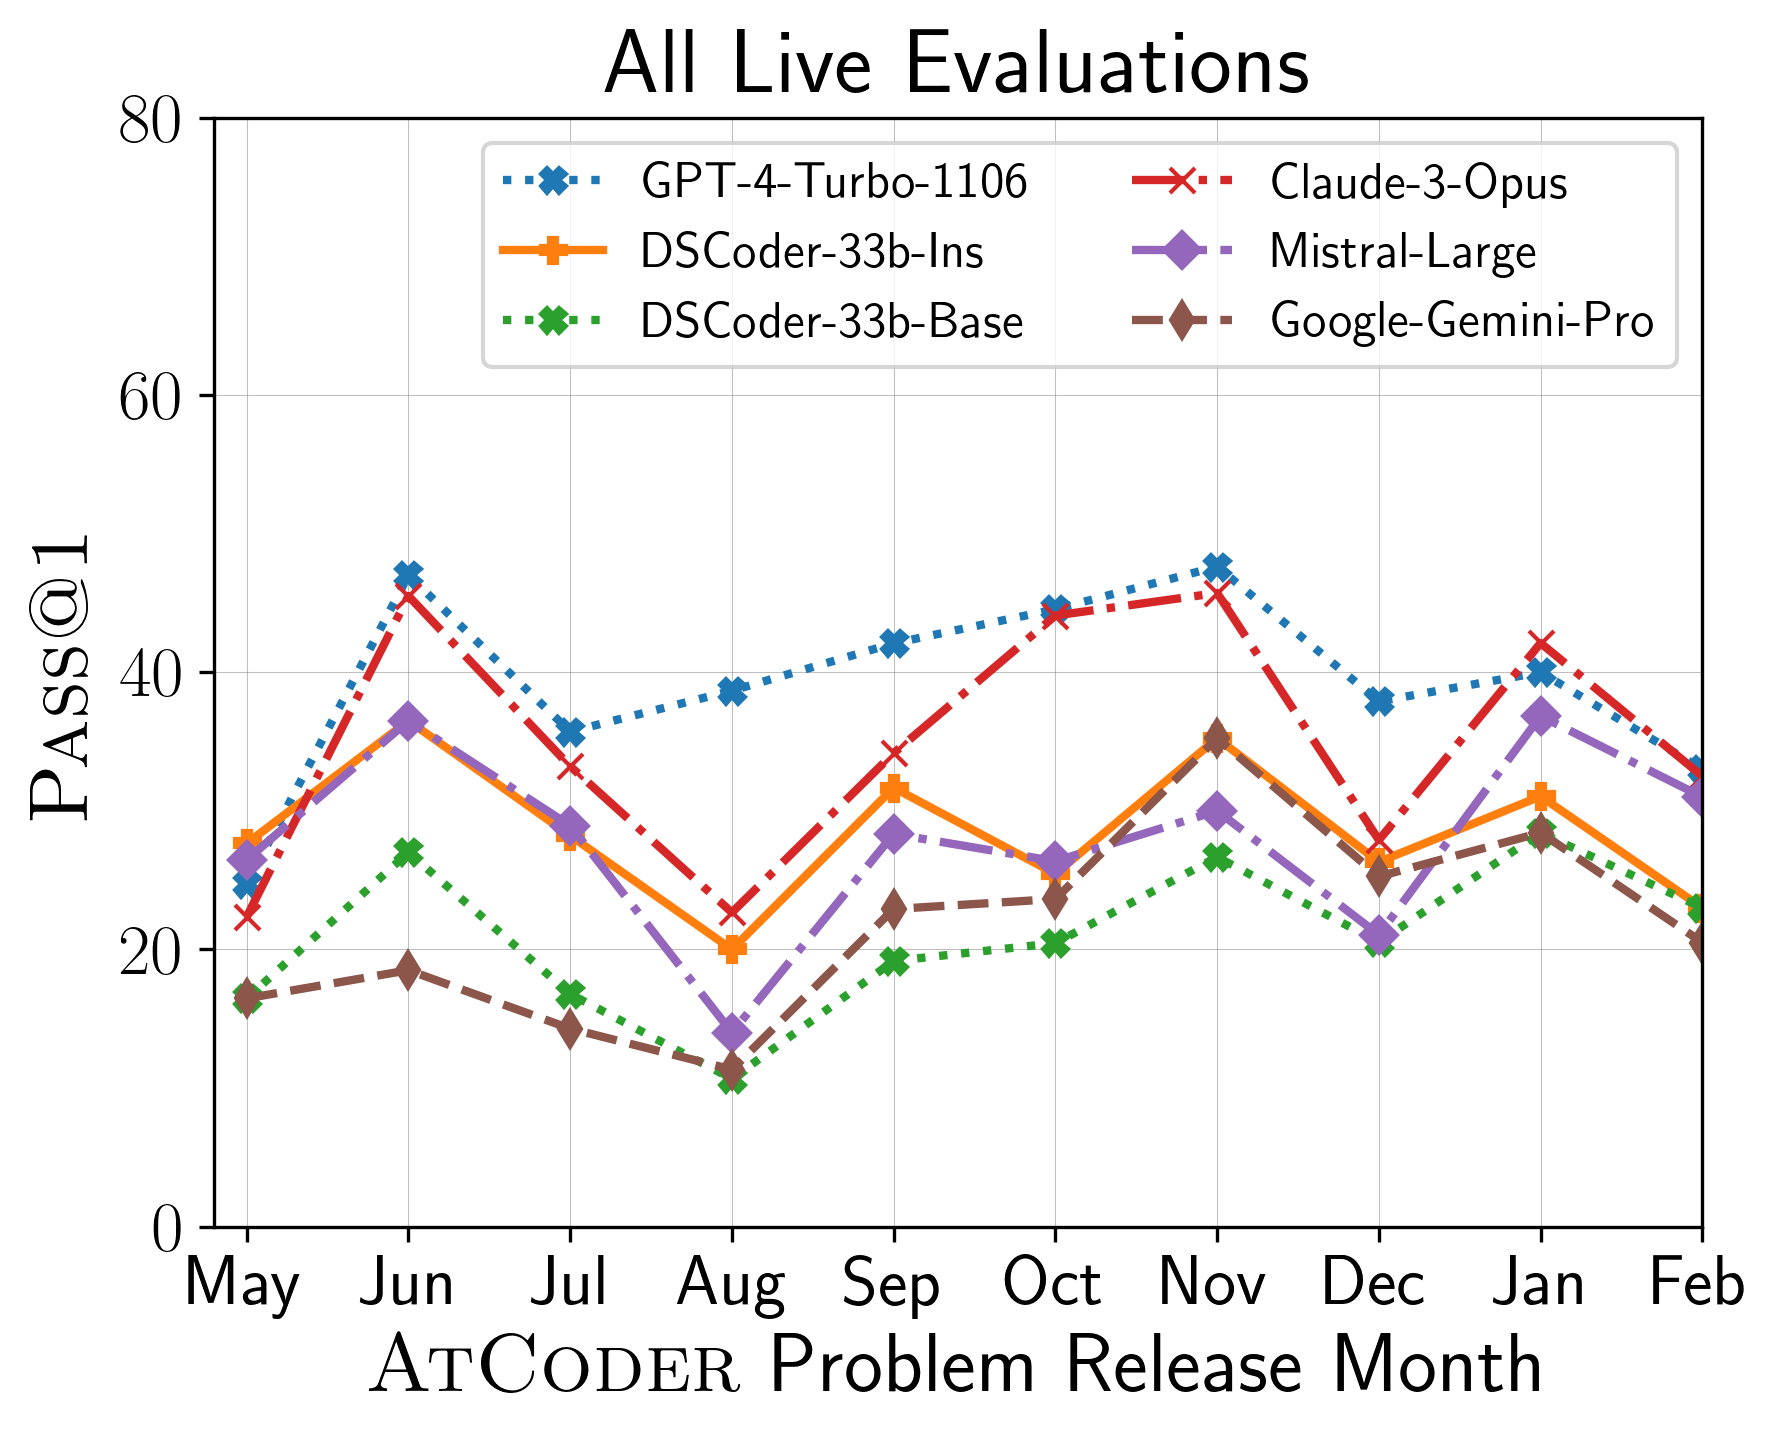
\includegraphics[width=0.49\linewidth]{figures/appendix/live_eval_custom_atcoder.png}
    \caption{Live evaluation over time for various models on code generation scenario in \livecodebench{}. We consider many recently released models and do not find significant performance variations across months except for \deepseekcode{} models.}
    \label{app:fig:contamination_all_models}
\end{figure}


\begin{figure}[!h]
    \centering
    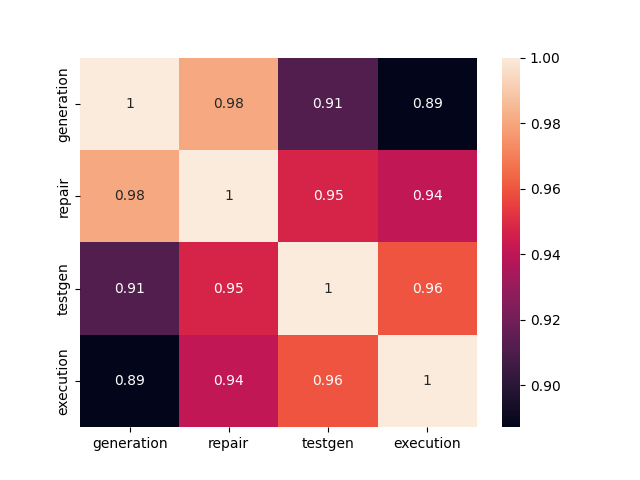
\includegraphics[width=0.49\linewidth]{figures/appendix/correlation_matrix.png}
    \caption{Correlations across different scenarios studied in \livecodebench{}}
    \label{app:fig:correlation_matrix}
\end{figure}



% Interestingly, in Figure~\ref{fig:he_vs_lcb} we find that while the base models had \textit{aligned} performances on 
% \lcb{}-Easy and \humanevalplus{} benchmarks, the fine-tuned models show a clearer performance 
% gap pointing out a lack of diverse fine-tuning data for open models.
% In contrast, closed-access models remain consistent across both benchmarks hinting at a more diverse fine-tuning data emloyed by them.


\noindent \textbf{Comparing Closed Models.}
We evaluate a range of closed (API access) models ranging from different model families 
like \gpts{}, \claudes{}, \gemini{}, and \mistral{}.
We find the \gptfourturbo{} and \claudeopus{} rank at the top across all scenarios followed by \mistrallarge{} and \claudesonnet{} models. 
Finally, \geminipro{} and \gptthreefiveturbo{} lie on the lower end of the models.
The relative differences between the models vary across the scenarios. 
For example, \gptfourturbo{} demonstrates remarkable improvement from self-repair ($24.5$\% to $36.9$\% on the \lcb{}-Medium problems) while \geminipro{} only improves from $8.5$\% to $9.4$\%.
Similarly, as identified above, \claudeopus{} and \mistrallarge{} perform considerably better on test output prediction and code execution scenarios. %\nj{add gemini pro flash}



\begin{figure}[!t]
    \centering
    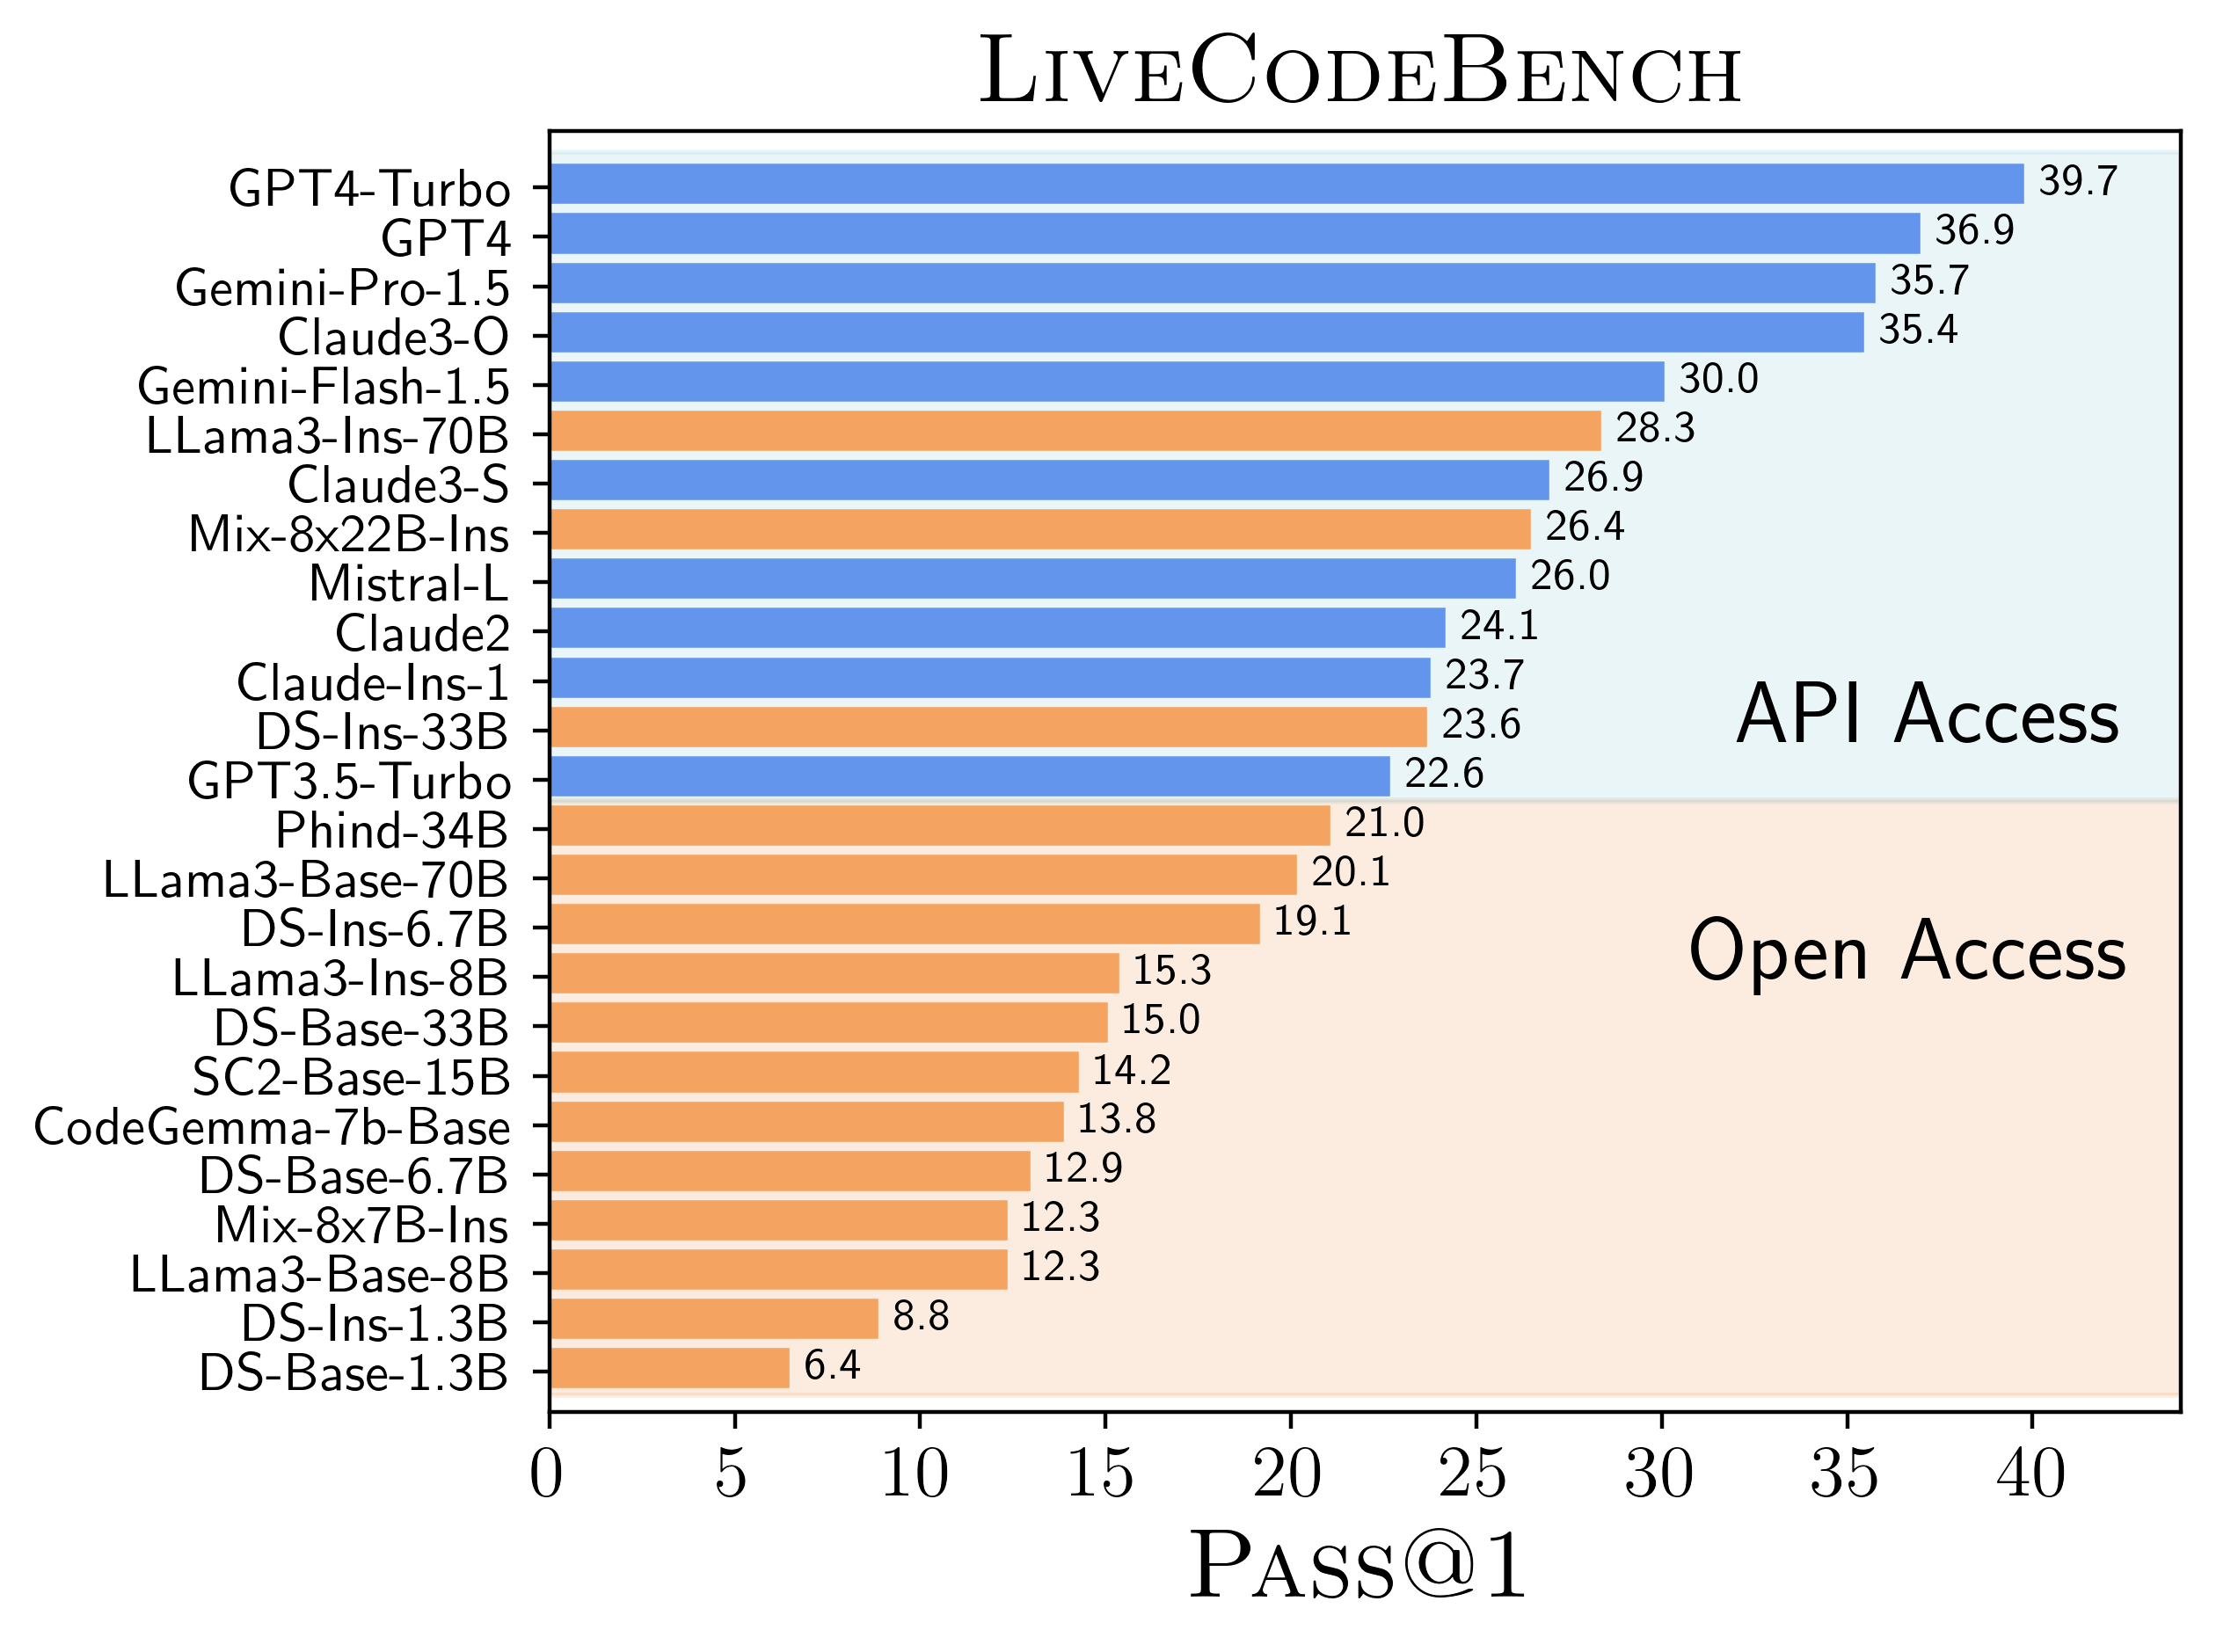
\includegraphics[width=0.7\linewidth]{figures/overview/lc_barchart.png}%

    \caption{
        Comparison of open access and (closed) API access models on \livecodebench{}-Easy 
        code generation scenario. We find that closed-access models consistently 
        outperform the open models with only strong instruction-tuned variants of $>30$\textsc{B}
        models (specifically \llamaB{70}, \mixtral and  \deepseekcodeB{33} models) crossing the performance gap.
        }
    \label{fig:oss}
\end{figure}


\subsubsection{C++ Results}
We evaluate model performances with C++ in Table~\ref{tab:cpp}. As we see, model performances roughly align across the two languages.

\begin{table}[!h]
    \centering
    \begin{tabular}{c|c}
    \hline
        \textbf{Model} & \passmetric{1} \\
    \hline
        GPT-4o & 49.8 \\
        Claude-3.5-Sonnet & 45.9 \\
    \hline
    \end{tabular}
    \caption{Results for models with C++ evaluations on the entire 713 \livecodebench{} problems}
    \label{tab:cpp}
\end{table}
